% Options for packages loaded elsewhere
% Options for packages loaded elsewhere
\PassOptionsToPackage{unicode}{hyperref}
\PassOptionsToPackage{hyphens}{url}
\PassOptionsToPackage{dvipsnames,svgnames,x11names}{xcolor}
%
\documentclass[
  spanish,
  letterpaper,
  DIV=11,
  numbers=noendperiod,
  oneside]{scrartcl}
\usepackage{xcolor}
\usepackage[left=1in,marginparwidth=2.0666666666667in,textwidth=4.1333333333333in,marginparsep=0.3in]{geometry}
\usepackage{amsmath,amssymb}
\setcounter{secnumdepth}{-\maxdimen} % remove section numbering
\usepackage{iftex}
\ifPDFTeX
  \usepackage[T1]{fontenc}
  \usepackage[utf8]{inputenc}
  \usepackage{textcomp} % provide euro and other symbols
\else % if luatex or xetex
  \usepackage{unicode-math} % this also loads fontspec
  \defaultfontfeatures{Scale=MatchLowercase}
  \defaultfontfeatures[\rmfamily]{Ligatures=TeX,Scale=1}
\fi
\usepackage{lmodern}
\ifPDFTeX\else
  % xetex/luatex font selection
\fi
% Use upquote if available, for straight quotes in verbatim environments
\IfFileExists{upquote.sty}{\usepackage{upquote}}{}
\IfFileExists{microtype.sty}{% use microtype if available
  \usepackage[]{microtype}
  \UseMicrotypeSet[protrusion]{basicmath} % disable protrusion for tt fonts
}{}
\makeatletter
\@ifundefined{KOMAClassName}{% if non-KOMA class
  \IfFileExists{parskip.sty}{%
    \usepackage{parskip}
  }{% else
    \setlength{\parindent}{0pt}
    \setlength{\parskip}{6pt plus 2pt minus 1pt}}
}{% if KOMA class
  \KOMAoptions{parskip=half}}
\makeatother
% Make \paragraph and \subparagraph free-standing
\makeatletter
\ifx\paragraph\undefined\else
  \let\oldparagraph\paragraph
  \renewcommand{\paragraph}{
    \@ifstar
      \xxxParagraphStar
      \xxxParagraphNoStar
  }
  \newcommand{\xxxParagraphStar}[1]{\oldparagraph*{#1}\mbox{}}
  \newcommand{\xxxParagraphNoStar}[1]{\oldparagraph{#1}\mbox{}}
\fi
\ifx\subparagraph\undefined\else
  \let\oldsubparagraph\subparagraph
  \renewcommand{\subparagraph}{
    \@ifstar
      \xxxSubParagraphStar
      \xxxSubParagraphNoStar
  }
  \newcommand{\xxxSubParagraphStar}[1]{\oldsubparagraph*{#1}\mbox{}}
  \newcommand{\xxxSubParagraphNoStar}[1]{\oldsubparagraph{#1}\mbox{}}
\fi
\makeatother


\usepackage{longtable,booktabs,array}
\usepackage{calc} % for calculating minipage widths
% Correct order of tables after \paragraph or \subparagraph
\usepackage{etoolbox}
\makeatletter
\patchcmd\longtable{\par}{\if@noskipsec\mbox{}\fi\par}{}{}
\makeatother
% Allow footnotes in longtable head/foot
\IfFileExists{footnotehyper.sty}{\usepackage{footnotehyper}}{\usepackage{footnote}}
\makesavenoteenv{longtable}
\usepackage{graphicx}
\makeatletter
\newsavebox\pandoc@box
\newcommand*\pandocbounded[1]{% scales image to fit in text height/width
  \sbox\pandoc@box{#1}%
  \Gscale@div\@tempa{\textheight}{\dimexpr\ht\pandoc@box+\dp\pandoc@box\relax}%
  \Gscale@div\@tempb{\linewidth}{\wd\pandoc@box}%
  \ifdim\@tempb\p@<\@tempa\p@\let\@tempa\@tempb\fi% select the smaller of both
  \ifdim\@tempa\p@<\p@\scalebox{\@tempa}{\usebox\pandoc@box}%
  \else\usebox{\pandoc@box}%
  \fi%
}
% Set default figure placement to htbp
\def\fps@figure{htbp}
\makeatother



\ifLuaTeX
\usepackage[bidi=basic]{babel}
\else
\usepackage[bidi=default]{babel}
\fi
% get rid of language-specific shorthands (see #6817):
\let\LanguageShortHands\languageshorthands
\def\languageshorthands#1{}


\setlength{\emergencystretch}{3em} % prevent overfull lines

\providecommand{\tightlist}{%
  \setlength{\itemsep}{0pt}\setlength{\parskip}{0pt}}



 


\KOMAoption{captions}{tableheading}
\makeatletter
\@ifpackageloaded{tcolorbox}{}{\usepackage[skins,breakable]{tcolorbox}}
\@ifpackageloaded{fontawesome5}{}{\usepackage{fontawesome5}}
\definecolor{quarto-callout-color}{HTML}{909090}
\definecolor{quarto-callout-note-color}{HTML}{0758E5}
\definecolor{quarto-callout-important-color}{HTML}{CC1914}
\definecolor{quarto-callout-warning-color}{HTML}{EB9113}
\definecolor{quarto-callout-tip-color}{HTML}{00A047}
\definecolor{quarto-callout-caution-color}{HTML}{FC5300}
\definecolor{quarto-callout-color-frame}{HTML}{acacac}
\definecolor{quarto-callout-note-color-frame}{HTML}{4582ec}
\definecolor{quarto-callout-important-color-frame}{HTML}{d9534f}
\definecolor{quarto-callout-warning-color-frame}{HTML}{f0ad4e}
\definecolor{quarto-callout-tip-color-frame}{HTML}{02b875}
\definecolor{quarto-callout-caution-color-frame}{HTML}{fd7e14}
\makeatother
\makeatletter
\@ifpackageloaded{caption}{}{\usepackage{caption}}
\AtBeginDocument{%
\ifdefined\contentsname
  \renewcommand*\contentsname{Tabla de contenidos}
\else
  \newcommand\contentsname{Tabla de contenidos}
\fi
\ifdefined\listfigurename
  \renewcommand*\listfigurename{Listado de Figuras}
\else
  \newcommand\listfigurename{Listado de Figuras}
\fi
\ifdefined\listtablename
  \renewcommand*\listtablename{Listado de Tablas}
\else
  \newcommand\listtablename{Listado de Tablas}
\fi
\ifdefined\figurename
  \renewcommand*\figurename{Figura}
\else
  \newcommand\figurename{Figura}
\fi
\ifdefined\tablename
  \renewcommand*\tablename{Tabla}
\else
  \newcommand\tablename{Tabla}
\fi
}
\@ifpackageloaded{float}{}{\usepackage{float}}
\floatstyle{ruled}
\@ifundefined{c@chapter}{\newfloat{codelisting}{h}{lop}}{\newfloat{codelisting}{h}{lop}[chapter]}
\floatname{codelisting}{Listado}
\newcommand*\listoflistings{\listof{codelisting}{Listado de Listados}}
\makeatother
\makeatletter
\makeatother
\makeatletter
\@ifpackageloaded{caption}{}{\usepackage{caption}}
\@ifpackageloaded{subcaption}{}{\usepackage{subcaption}}
\makeatother
\makeatletter
\@ifpackageloaded{sidenotes}{}{\usepackage{sidenotes}}
\@ifpackageloaded{marginnote}{}{\usepackage{marginnote}}
\makeatother
\usepackage{bookmark}
\IfFileExists{xurl.sty}{\usepackage{xurl}}{} % add URL line breaks if available
\urlstyle{same}
\hypersetup{
  pdftitle={Práctica 8: BIM semántico},
  pdflang={es},
  colorlinks=true,
  linkcolor={blue},
  filecolor={Maroon},
  citecolor={Blue},
  urlcolor={Blue},
  pdfcreator={LaTeX via pandoc}}


\title{Práctica 8: BIM semántico}
\author{}
\date{}
\begin{document}
\maketitle


{ \textasciitilde8 min de lectura }

\subsection{Objetivos de la práctica}\label{objetivos-de-la-pruxe1ctica}

En esta práctica trabajaremos con un mismo edificio en dos
representaciones complementarias: un modelo BIM (\emph{Building
Information Modeling}) en formato IFC (\emph{Industry Foundation
Classes}) y una versión semántica en OWL (\emph{Web Ontology Language}).
Al finalizar, deberías ser capaz de:

\begin{itemize}
\tightlist
\item
  Entender qué aporta BIM como sistema de organización de información de
  un edificio.
\item
  Explorar un modelo IFC con un visor BIM y localizar elementos
  concretos.
\item
  Abrir una ontología en \emph{Protégé} y recorrer sus clases,
  propiedades e individuos.
\item
  Realizar consultas semánticas con un razonador para recuperar
  información del modelo.
\end{itemize}

\subsection{Introducción a BIM}\label{introducciuxf3n-a-bim}

\begin{figure}

\begin{minipage}{0.58\linewidth}
El \textbf{modelado de información de construcción} (\textbf{BIM},
\emph{Building Information Modeling}) es una forma de representar
digitalmente un edificio y la información asociada a sus elementos. No
se trata solo de una maqueta 3D: un modelo BIM también puede describir
materiales, relaciones espaciales, identificadores, propiedades
geométricas y datos útiles para diseño, obra, mantenimiento y
explotación.Esta manera de trabajar resulta especialmente valiosa porque
reúne en un mismo modelo información que normalmente estaría dispersa en
planos, tablas, memorias y documentos técnicos. Por eso BIM se ha
convertido en una pieza clave en la digitalización del sector de la
construcción.\end{minipage}%
%
\begin{minipage}{0.42\linewidth}

\begin{figure}[H]

\centering{

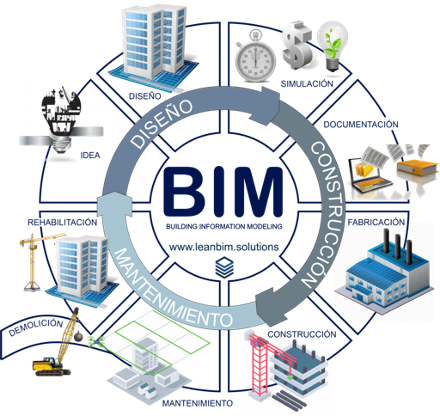
\includegraphics[width=1\linewidth,height=\textheight,keepaspectratio]{../resources/practica8/bim1.png}

}

\caption{\label{fig-bim}Esquema general del flujo de trabajo BIM.
Fuente: \emph{BIMCloud}.}

\end{figure}%

\end{minipage}%

\end{figure}%

El valor de BIM se aprecia mejor cuando pensamos en el \textbf{ciclo de
vida} completo de la edificación. La misma información puede servir para
coordinar el proyecto, detectar interferencias, planificar fases de obra
o consultar características de un elemento una vez construido.

\begin{figure}

\centering{

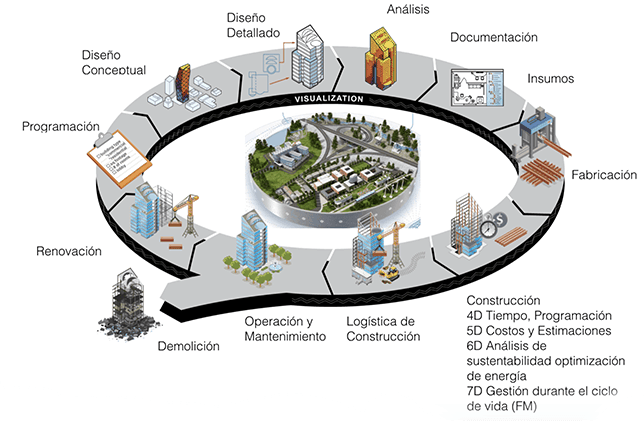
\includegraphics[width=0.8\linewidth,height=\textheight,keepaspectratio]{../resources/practica8/bim2.png}

}

\caption{\label{fig-bim-cycle}Ciclo de vida de la edificación y papel
del modelo BIM. Fuente: \emph{ip21ingenieria}.}

\end{figure}%

En el siguiente vídeo de \emph{Autodesk Building Solutions} se explica
de forma sencilla qué es BIM y qué ventajas aporta a lo largo del ciclo
de vida de un edificio:

\url{https://www.youtube.com/watch?v=suNadRnHy-Un}

\begin{tcolorbox}[enhanced jigsaw, colbacktitle=quarto-callout-note-color!10!white, coltitle=black, leftrule=.75mm, toprule=.15mm, rightrule=.15mm, breakable, bottomrule=.15mm, colframe=quarto-callout-note-color-frame, bottomtitle=1mm, arc=.35mm, opacitybacktitle=0.6, titlerule=0mm, colback=white, title=\textcolor{quarto-callout-note-color}{\faInfo}\hspace{0.5em}{Idea clave}, toptitle=1mm, left=2mm, opacityback=0]

En esta práctica no vamos a modelar un edificio desde cero. Vamos a
aprender a \textbf{leer} un modelo BIM y a \textbf{consultar} su
información, primero con un visor IFC (\emph{Industry Foundation
Classes}) y después con herramientas semánticas.

\end{tcolorbox}

\subsection{Material de trabajo}\label{material-de-trabajo}

Utilizaremos los siguientes ficheros:

\begin{itemize}
\tightlist
\item
  \href{../resources/practica8/Duplex.ifc}{Duplex.ifc}, que contiene el
  modelo BIM original del apartamento dúplex en formato IFC
  (\emph{Industry Foundation Classes}).
\item
  \href{../resources/practica8/Duplex.owl}{Duplex.owl}, que contiene una
  versión semántica del mismo modelo en lenguaje \textbf{OWL} (\emph{Web
  Ontology Language}).
\item
  \href{../resources/practica8/beo.owl}{beo.owl} y
  \href{../resources/practica8/bot.owl}{bot.owl}, que pueden ser
  necesarios si \emph{Protégé} te pide resolver manualmente algunas
  importaciones.
\end{itemize}

Como software de apoyo utilzaremos
\href{https://bimvision.eu}{BIMvision} para visualizar el IFC y
\href{http://protege.stanford.edu}{Protégé} para explorar la ontología.

\subsection{Ejercicio 1: explorar el modelo
IFC}\label{ejercicio-1-explorar-el-modelo-ifc}

El primer paso es abrir \texttt{Duplex.ifc} en \textbf{BIMvision}. El
objetivo no es todavía hacer consultas complejas, sino familiarizarse
con el edificio, sus plantas y la forma en que cada elemento aparece
identificado en el modelo.

\begin{figure}

\centering{

\pandocbounded{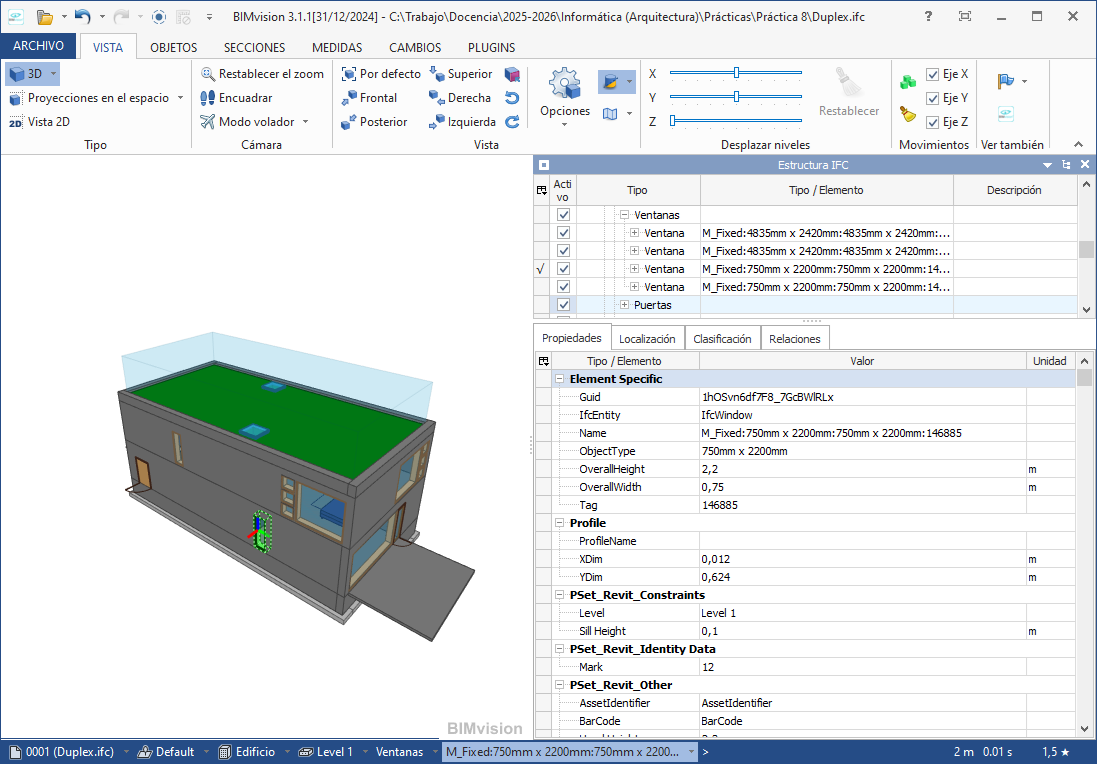
\includegraphics[keepaspectratio]{../resources/practica8/duplex_bimvision.png}}

}

\caption{\label{fig-viewer}Modelo Duplex abierto en BIMvision.}

\end{figure}%

\begin{tcolorbox}[enhanced jigsaw, colbacktitle=quarto-callout-tip-color!10!white, coltitle=black, leftrule=.75mm, toprule=.15mm, rightrule=.15mm, breakable, bottomrule=.15mm, colframe=quarto-callout-tip-color-frame, bottomtitle=1mm, arc=.35mm, opacitybacktitle=0.6, titlerule=0mm, colback=white, title=\textcolor{quarto-callout-tip-color}{\faLightbulb}\hspace{0.5em}{Qué debes observar}, toptitle=1mm, left=2mm, opacityback=0]

Empieza por recorrer la planta baja y la planta superior, y acostúmbrate
a seleccionar elementos individuales. Fíjate en cómo el visor muestra
sus nombres, identificadores y propiedades básicas.

\end{tcolorbox}

\begin{tcolorbox}[enhanced jigsaw, colbacktitle=quarto-callout-note-color!10!white, coltitle=black, leftrule=.75mm, toprule=.15mm, rightrule=.15mm, breakable, bottomrule=.15mm, colframe=quarto-callout-note-color-frame, bottomtitle=1mm, arc=.35mm, opacitybacktitle=0.6, titlerule=0mm, colback=white, title=\textcolor{quarto-callout-note-color}{\faInfo}\hspace{0.5em}{🧠 Encuentra elementos}, toptitle=1mm, left=2mm, opacityback=0]

Durante esta primera exploración, responde a las siguientes preguntas:

\begin{itemize}
\tightlist
\item
  \textbf{¿Cuántas ventanas hay en el modelo?}
\item
  \textbf{¿Qué identificador tiene cada una?}
\item
  \textbf{¿Qué altura y qué anchura tiene cada ventana?}
\end{itemize}

\end{tcolorbox}

\subsection{Del IFC al modelo
semántico}\label{del-ifc-al-modelo-semuxe1ntico}

El siguiente paso consiste en pasar de una representación BIM
convencional a una representación \textbf{semántica}. En lugar de
trabajar solamente con geometría y propiedades dentro de un visor, vamos
a describir el edificio mediante clases, propiedades e individuos
conectados entre sí en una ontología.

En esta práctica no es necesario que hagas la conversión por tu cuenta,
porque el fichero \texttt{Duplex.owl} ya está preparado. Aun así,
conviene entender de dónde sale: se ha generado a partir del IFC usando
\href{https://github.com/jyrkioraskari/IFCtoLBD/releases/tag/2.43.5}{IFCtoLBD
2.43.5}, una herramienta que transforma modelos IFC en datos enlazados
reutilizando vocabularios existentes del ámbito de la construcción.
{\marginnote{\begin{footnotesize}El fichero \texttt{Duplex.owl} se ha
generado con la configuración \textbf{BOT + PRODUCT + PROPS, Level L1}.
Además, se han eliminado manualmente las referencias a dos ontologías
externas para simplificar la práctica.\end{footnotesize}}}

\subsection{Ejercicio 2: abrir la ontología en
Protégé}\label{ejercicio-2-abrir-la-ontologuxeda-en-protuxe9guxe9}

Para abrir \texttt{Duplex.owl} usaremos \textbf{Protégé}, un editor de
ontologías gratuito y disponible para varios sistemas operativos. No
requiere una instalación compleja: basta con descargar el archivo
comprimido, descomprimirlo y ejecutar la aplicación.

La interfaz puede cambiar ligeramente según la versión de
\emph{Protégé}, pero la idea general es siempre la misma: pasar de la
estructura conceptual a los elementos concretos del edificio.

Una vez abierto el fichero, encontrarás varias vistas desde las que
puedes navegar por la ontología. Debajo del título de la ontología,
\emph{converters}, puedes encontrar una pestaña llamada
\textbf{\emph{Entities}} que te permitirá acceder a las siguientes
categorías:

\begin{itemize}
\tightlist
\item
  \textbf{Classes}, para ver la jerarquía de clases del dominio.
\item
  \textbf{Object properties}, para ver propiedades cuyo valor es otro
  objeto o individuo.
\item
  \textbf{Data properties}, para ver propiedades cuyo valor es un dato
  literal.
\item
  \textbf{Individuals}, para ver las instancias concretas del modelo.
\end{itemize}

La Figura~\ref{fig-protege} muestra el resultado de seleccionar
\textbf{\emph{Clases}} y, concretamente, \textbf{\emph{Edificio}}.
Podeis observar cómo la interfaz nos muestra que
\textbf{\emph{Edificio}} es una subclase de \textbf{\emph{Zona}}.

\begin{figure}

\centering{

\pandocbounded{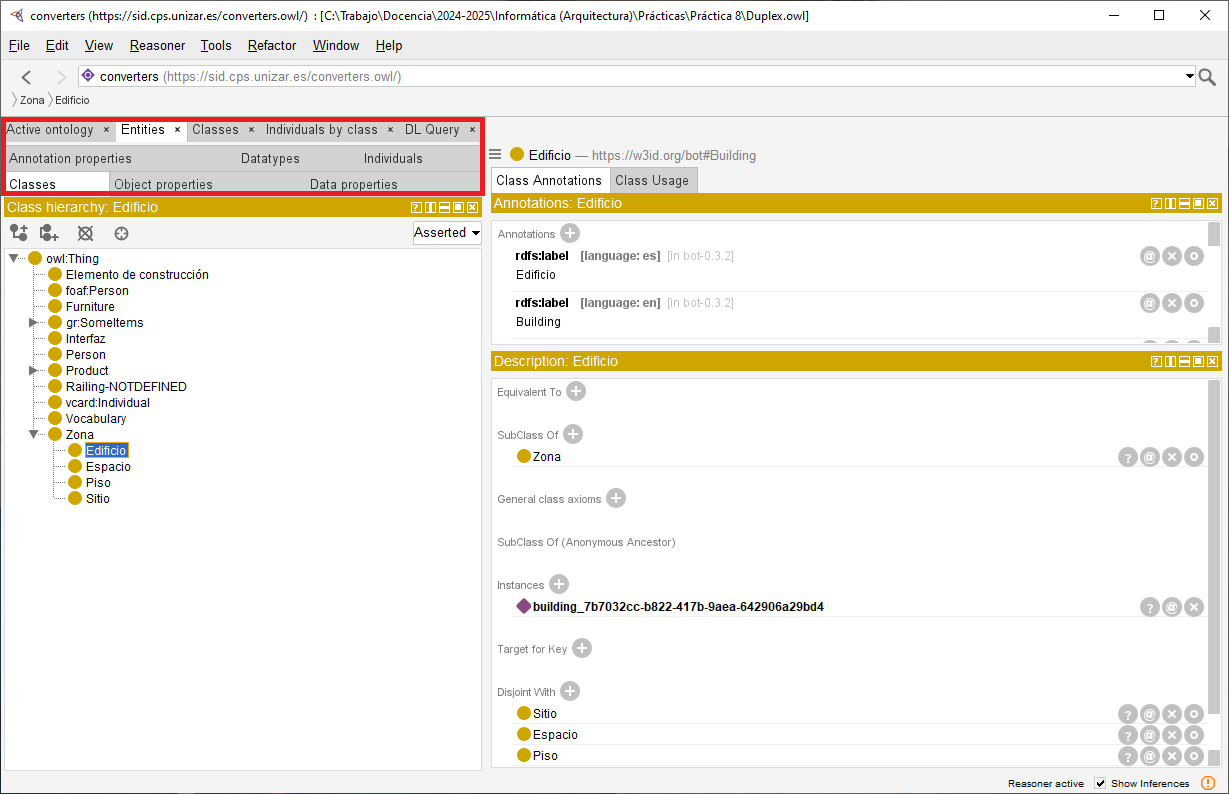
\includegraphics[keepaspectratio]{../resources/practica8/protege_overview.png}}

}

\caption{\label{fig-protege}Jerarquía de clases y detalle de una clase
en Protégé.}

\end{figure}%

Puedes encontrar una pequeña introducción a la interfaz de
\emph{Protégé} en el siguiente vídeo, aunque no está orientado a nuestro
mismo modelo, por lo que no es necesario seguirlo al pie de la letra:

\url{https://drive.google.com/file/d/1eHHxYrJRiQZni_7KKrtRFqu5KEwk9omW}

\begin{tcolorbox}[enhanced jigsaw, colbacktitle=quarto-callout-tip-color!10!white, coltitle=black, leftrule=.75mm, toprule=.15mm, rightrule=.15mm, breakable, bottomrule=.15mm, colframe=quarto-callout-tip-color-frame, bottomtitle=1mm, arc=.35mm, opacitybacktitle=0.6, titlerule=0mm, colback=white, title=\textcolor{quarto-callout-tip-color}{\faLightbulb}\hspace{0.5em}{Si faltan importaciones}, toptitle=1mm, left=2mm, opacityback=0]

En algunas versiones de \emph{Protégé}, las ontologías importadas se
descargan automáticamente desde Internet. En otras, tendremos que
resolver manualmente las importaciones. En este último caso, en
\texttt{Active\ ontology\ \textgreater{}\ Ontology\ imports} pinchamos
en el botón \texttt{+} para añadir los ficheros
\href{../resources/practica8/beo.owl}{beo.owl} y
\href{../resources/practica8/bot.owl}{⬇️ bot.owl}.

\end{tcolorbox}

También debes tener en cuenta que muchas entidades tienen
\textbf{etiquetas en varios idiomas}. Dependiendo de la configuración de
tu equipo, \emph{Protégé} puede mostrar nombres en castellano o en
inglés. Por ejemplo, la clase
\texttt{Edificio\ ‐\ http://w3id.org/bot/Building} tiene etiquetas
\texttt{Building}, \texttt{Edificio}, etc. En este guion se asume que
las etiquetas se muestran en castellano siempre que sea posible.

\subsubsection{Qué debes localizar}\label{quuxe9-debes-localizar}

Dentro de la ontología, localiza:

\begin{itemize}
\tightlist
\item
  \textbf{La clase que permite representar las ventanas}.
\item
  \textbf{Las propiedades que representan la altura y la anchura de una
  ventana}.
\item
  \textbf{Una ventana concreta y los valores de sus propiedades}.
\end{itemize}

Comprueba además si esos valores coinciden con los que viste en el visor
IFC durante el ejercicio anterior.

💡 Solución orientativa: clases

\begin{figure}

\centering{

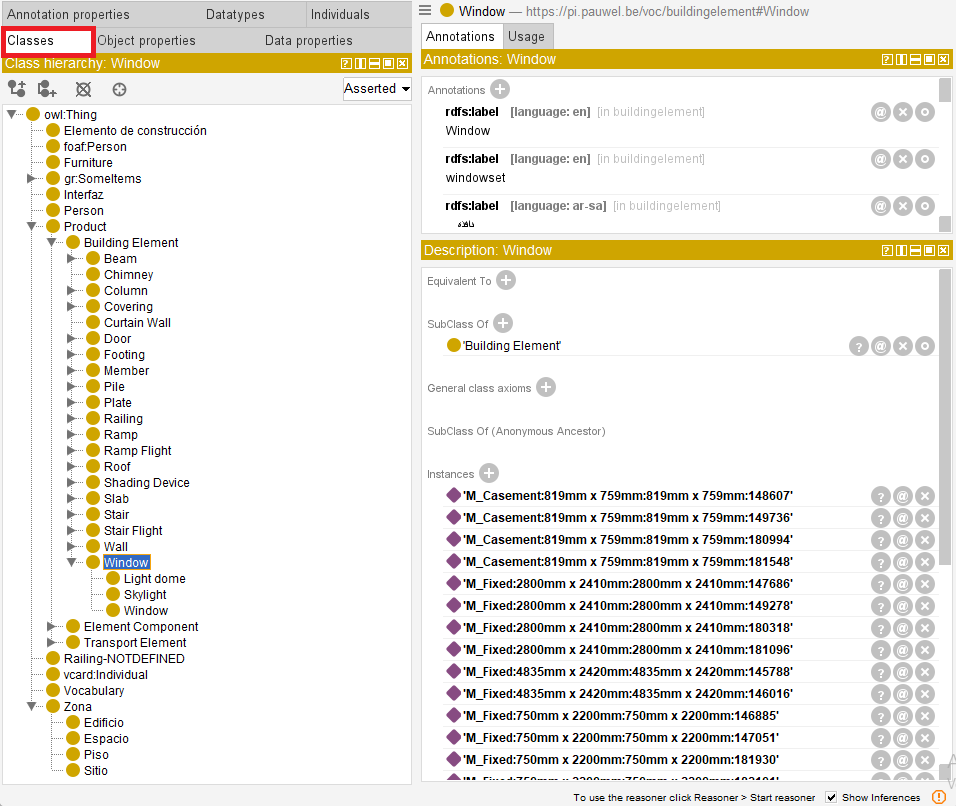
\includegraphics[width=1\linewidth,height=\textheight,keepaspectratio]{../resources/practica8/classes.png}

}

\caption{\label{fig-classes-solution}Jerarquía de clases para localizar
la entidad de ventana.}

\end{figure}%

💡 Solución orientativa: propiedades

\begin{figure}

\centering{

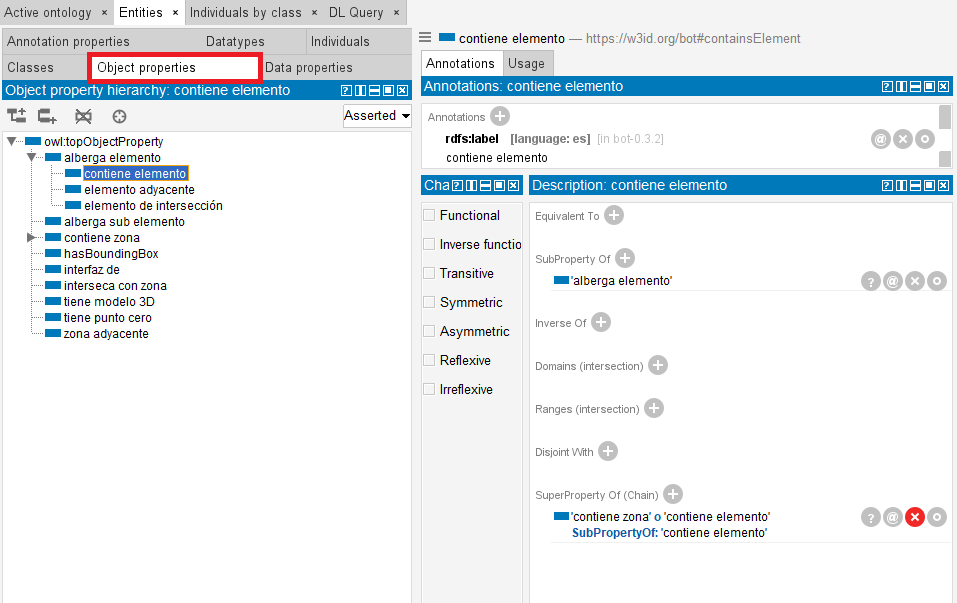
\includegraphics[width=1\linewidth,height=\textheight,keepaspectratio]{../resources/practica8/property1.png}

}

\caption{\label{fig-property-object}Propiedades de objeto relacionadas
con los elementos del modelo.}

\end{figure}%

\begin{figure}

\centering{

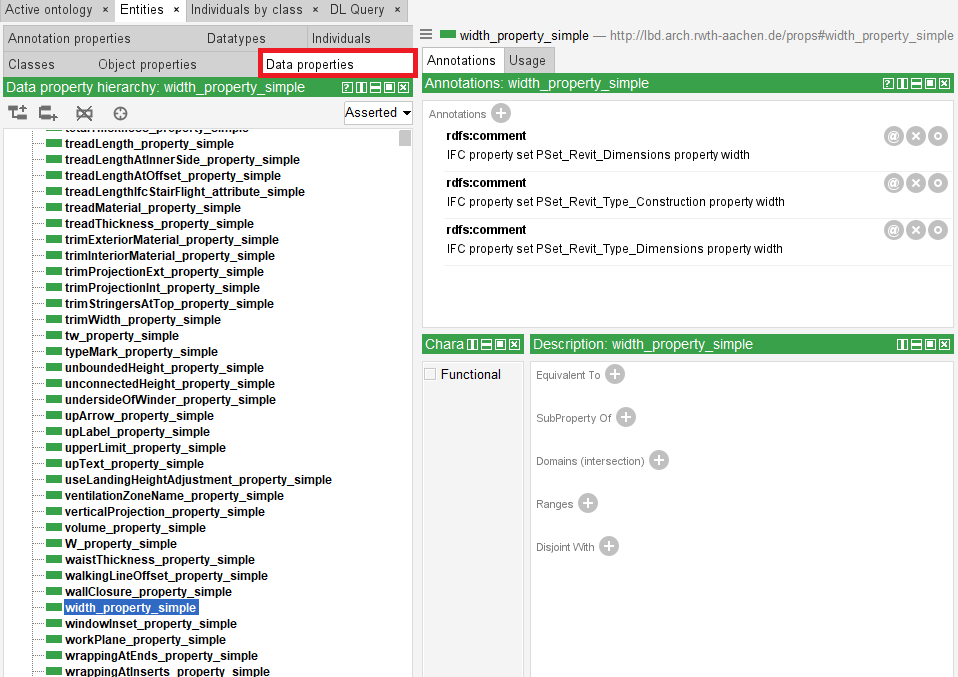
\includegraphics[width=1\linewidth,height=\textheight,keepaspectratio]{../resources/practica8/property2.png}

}

\caption{\label{fig-property-data}Propiedades de datos para recuperar
medidas y otros valores literales.}

\end{figure}%

💡 Solución orientativa: individuos

\begin{figure}

\centering{

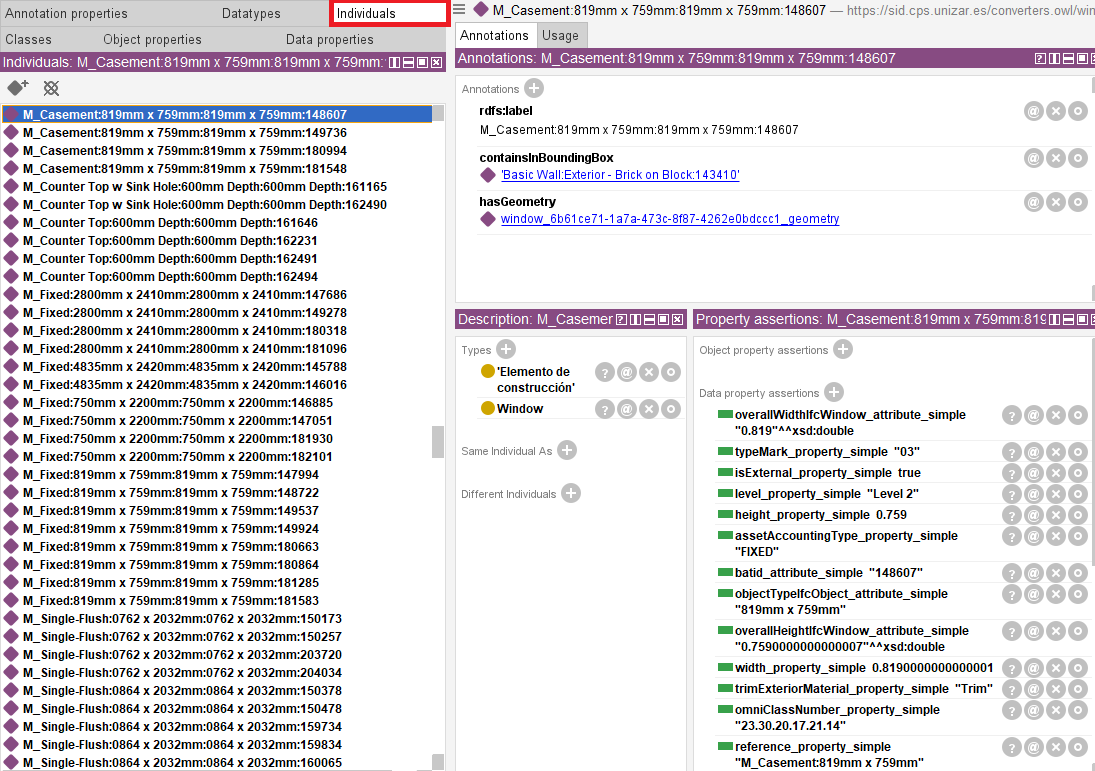
\includegraphics[width=1\linewidth,height=\textheight,keepaspectratio]{../resources/practica8/individuals.png}

}

\caption{\label{fig-individuals-solution}Exploración de individuos
concretos dentro de la ontología.}

\end{figure}%

\subsection{Ejercicio 3: razonamiento e
inferencia}\label{ejercicio-3-razonamiento-e-inferencia}

Una de las ventajas de trabajar con ontologías es que no solo podemos
leer datos explícitos, sino también \textbf{inferir} información nueva a
partir de la estructura del modelo y de las restricciones definidas en
la ontología.

Para ello, activa un razonador desde el menú superior \textbf{Reasoner}.
En esta práctica se recomienda utilizar \textbf{HermiT}. Inicia el
razonador mediante \texttt{Reasoner\ \textgreater{}\ Start\ reasoner}.
Una vez cargado, podrás abrir la pestaña \textbf{DL Query} para lanzar
consultas sobre clases e individuos.

Si en algún momento actualizamos la ontología, tendremos que utilizar la
opción \textbf{Synchronize reasoner} para que el razonador actualice su
información y pueda responder a las consultas correctamente.

\subsubsection{Consultas propuestas}\label{consultas-propuestas}

A través de la pestaña \textbf{\emph{DL Query}}, recupera las instancias
de la clase que representa las \textbf{ventanas}. Pinchando en alguna de
ellas, puedes ver los valores de las propiedades (tanto los originales
como los inferidos por el razonador, si los hubiera).

Con el razonador activo, realiza las siguientes comprobaciones:

\begin{itemize}
\tightlist
\item
  \textbf{Recupera las instancias de la clase que representa las
  ventanas}.
\item
  \textbf{Recupera las superclases} de esa clase.
\item
  \textbf{Recupera las instancias de alguna de esas superclases para
  comprobar si el razonador también devuelve instancias indirectas}.
\item
  \textbf{Vuelve a consultar las instancias de la clase de ventanas y
  haz clic en el símbolo \texttt{?} de alguna de ellas para ver al menos
  una explicación}.
\end{itemize}

\begin{tcolorbox}[enhanced jigsaw, colbacktitle=quarto-callout-note-color!10!white, coltitle=black, leftrule=.75mm, toprule=.15mm, rightrule=.15mm, breakable, bottomrule=.15mm, colframe=quarto-callout-note-color-frame, bottomtitle=1mm, arc=.35mm, opacitybacktitle=0.6, titlerule=0mm, colback=white, title=\textcolor{quarto-callout-note-color}{\faInfo}\hspace{0.5em}{Pista}, toptitle=1mm, left=2mm, opacityback=0]

En muchas instalaciones, las consultas se escriben con los nombres
cortos en inglés, por ejemplo \texttt{Window}, aunque en la interfaz
veas etiquetas en castellano.

\end{tcolorbox}

💡 Ejemplo orientativo: consulta sobre escaleras

\begin{figure}

\centering{

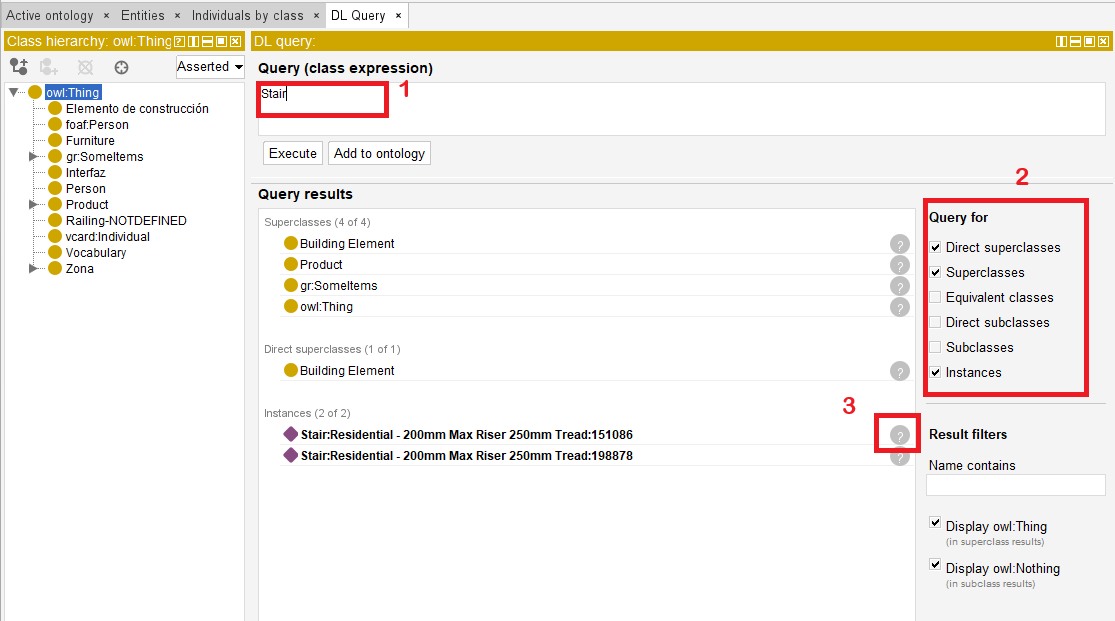
\includegraphics[width=0.75\linewidth,height=\textheight,keepaspectratio]{../resources/practica8/stairs_example_DL.png}

}

\caption{\label{fig-stairs-dl}Ejemplo de consulta DL en Protégé.}

\end{figure}%

\begin{figure}

\centering{

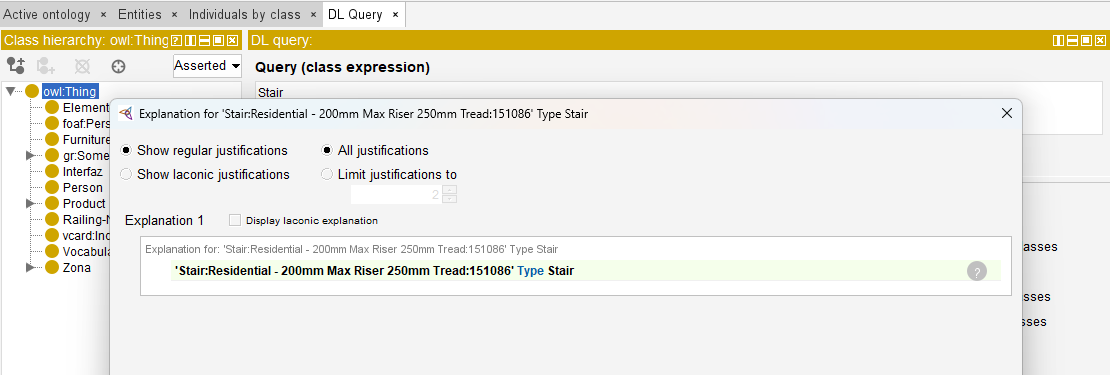
\includegraphics[width=0.7\linewidth,height=\textheight,keepaspectratio]{../resources/practica8/stair_explanation.png}

}

\caption{\label{fig-stairs-explanation}Ejemplo de explicación ofrecida
por el razonador.}

\end{figure}%

\subsection{Ejercicio 4: consultas más
expresivas}\label{ejercicio-4-consultas-muxe1s-expresivas}

Una vez dominadas las consultas básicas, podemos construir expresiones
más ricas combinando clases y propiedades. Esto permite formular
preguntas que no se reducen a ``dame todas las instancias de una
clase'', sino a ``dame todos los elementos que cumplan una determinada
condición''.

Por ejemplo, lanza la siguiente consulta:

\texttt{Espacio\ and\ \textquotesingle{}elemento\ adyacente\textquotesingle{}\ some\ Window}

Esa expresión representa el conjunto de espacios que tienen al menos un
elemento adyacente que pertenece a la clase \textbf{Window}.

\begin{tcolorbox}[enhanced jigsaw, colbacktitle=quarto-callout-note-color!10!white, coltitle=black, leftrule=.75mm, toprule=.15mm, rightrule=.15mm, breakable, bottomrule=.15mm, colframe=quarto-callout-note-color-frame, bottomtitle=1mm, arc=.35mm, opacitybacktitle=0.6, titlerule=0mm, colback=white, title=\textcolor{quarto-callout-note-color}{\faInfo}\hspace{0.5em}{Pista}, toptitle=1mm, left=2mm, opacityback=0]

A medidas que escribes la consulta, \emph{Protégé} te ofrece sugerencias
de autocompletado para las clases y propiedades. Si no recuerdas el
nombre exacto, puedes aprovechar esa función para construir la consulta.
Si no aparecen las sugerencias a medida que escribes, puedes pulsar
\texttt{Ctrl\ +\ Space} para forzar que se muestren.

\end{tcolorbox}

\begin{tcolorbox}[enhanced jigsaw, colbacktitle=quarto-callout-note-color!10!white, coltitle=black, leftrule=.75mm, toprule=.15mm, rightrule=.15mm, breakable, bottomrule=.15mm, colframe=quarto-callout-note-color-frame, bottomtitle=1mm, arc=.35mm, opacitybacktitle=0.6, titlerule=0mm, colback=white, title=\textcolor{quarto-callout-note-color}{\faInfo}\hspace{0.5em}{🧠 Explora los resultados}, toptitle=1mm, left=2mm, opacityback=0]

Responde a estas preguntas:

\begin{itemize}
\tightlist
\item
  \textbf{¿Cuántos individuos recupera la consulta?}
\item
  \textbf{¿Qué tipo de espacios son?}
\item
  \textbf{¿Coincide ese resultado con lo que esperarías al observar el
  edificio en el visor IFC?}
\end{itemize}

\end{tcolorbox}

\subsection{Ejercicio 5: provocar una
inconsistencia}\label{ejercicio-5-provocar-una-inconsistencia}

Si una ontología se vuelve \textbf{inconsistente}, el razonador ya no
puede trabajar correctamente con ella. En ese caso, \emph{Protégé}
muestra un aviso y permite abrir una explicación para entender qué
axiomas están entrando en conflicto.

En este ejercicio vamos a provocar una inconsistencia de forma
controlada. La idea es declarar como \textbf{funcional} la propiedad que
representa la altura de una ventana y, después, asignar a una misma
ventana dos valores distintos para esa altura.

\subsubsection{Pasos sugeridos}\label{pasos-sugeridos}

\begin{enumerate}
\def\labelenumi{\arabic{enumi}.}
\tightlist
\item
  Localiza la propiedad de datos que representa la altura.
\item
  Márcala como \textbf{Functional}.
\item
  Busca una ventana concreta en \textbf{Individuals}.
\item
  Añade una segunda afirmación de tipo \textbf{Data property assertion}
  con un valor distinto del original, por ejemplo \texttt{1234}.
\item
  Sincroniza el razonador y observa el error de inconsistencia.
\end{enumerate}

\begin{tcolorbox}[enhanced jigsaw, colbacktitle=quarto-callout-warning-color!10!white, coltitle=black, leftrule=.75mm, toprule=.15mm, rightrule=.15mm, breakable, bottomrule=.15mm, colframe=quarto-callout-warning-color-frame, bottomtitle=1mm, arc=.35mm, opacitybacktitle=0.6, titlerule=0mm, colback=white, title=\textcolor{quarto-callout-warning-color}{\faExclamationTriangle}\hspace{0.5em}{Recomendación}, toptitle=1mm, left=2mm, opacityback=0]

Haz este ejercicio sobre una copia de trabajo del fichero si quieres
conservar \texttt{Duplex.owl} sin cambios al terminar la práctica.

\end{tcolorbox}

Solución orientativa: inconsistencia

\begin{figure}

\centering{

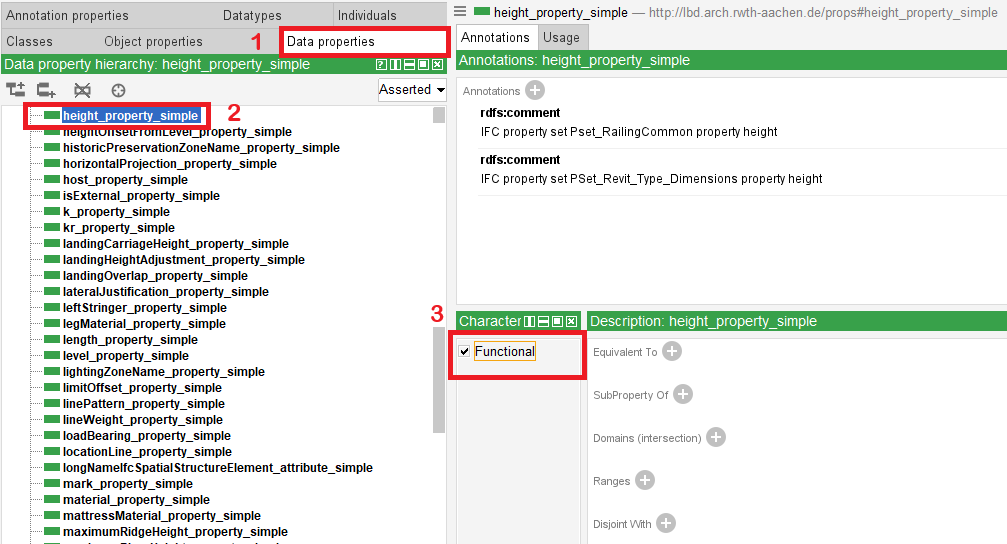
\includegraphics[width=1\linewidth,height=\textheight,keepaspectratio]{../resources/practica8/functional_property.png}

}

\caption{\label{fig-functional}Marcar la propiedad como funcional.}

\end{figure}%

\begin{figure}

\centering{

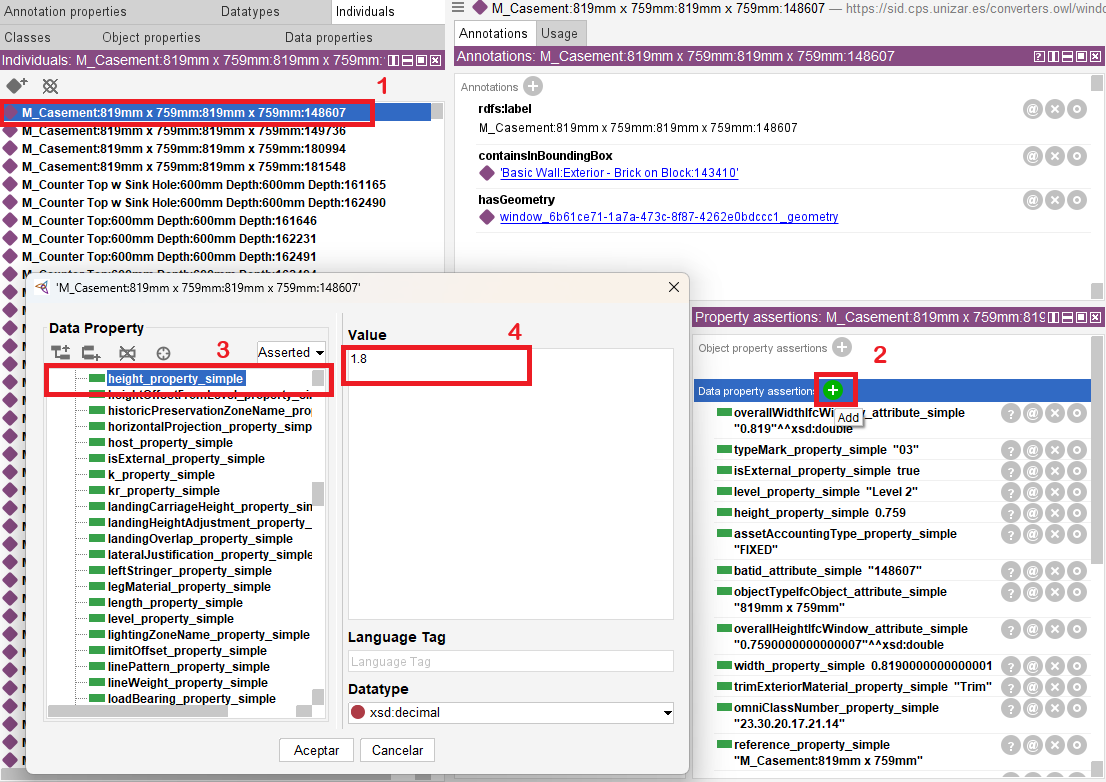
\includegraphics[width=1\linewidth,height=\textheight,keepaspectratio]{../resources/practica8/property_value.png}

}

\caption{\label{fig-property-value}Añadir un segundo valor incompatible
para la propiedad.}

\end{figure}%

\begin{figure}

\centering{

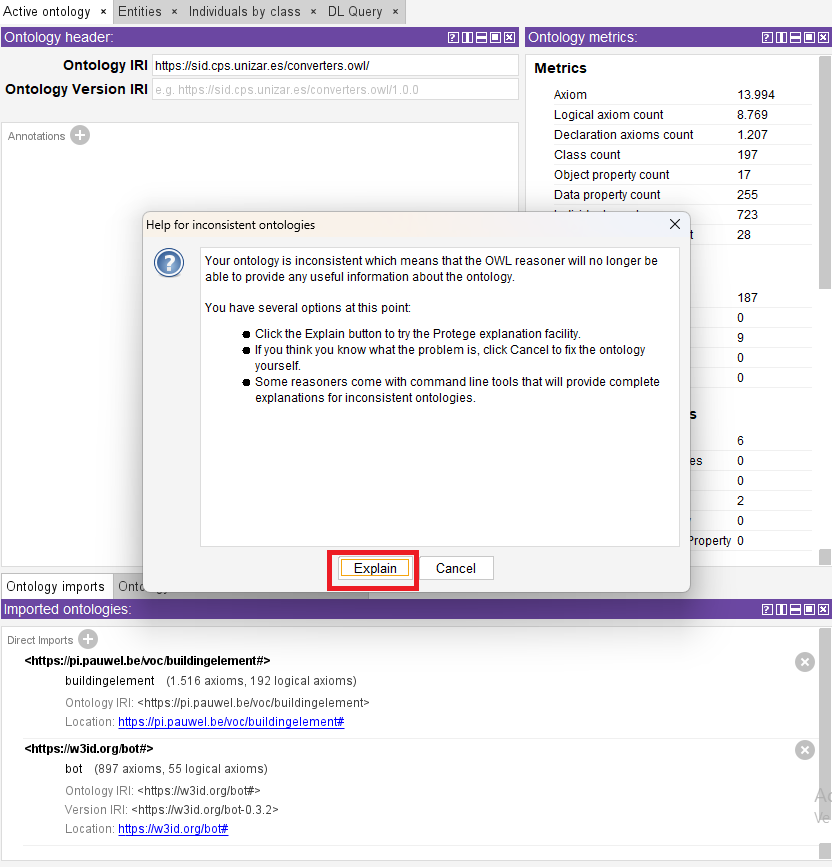
\includegraphics[width=1\linewidth,height=\textheight,keepaspectratio]{../resources/practica8/explain.png}

}

\caption{\label{fig-explain}Aviso de inconsistencia y acceso a la
explicación.}

\end{figure}%

\begin{figure}

\centering{

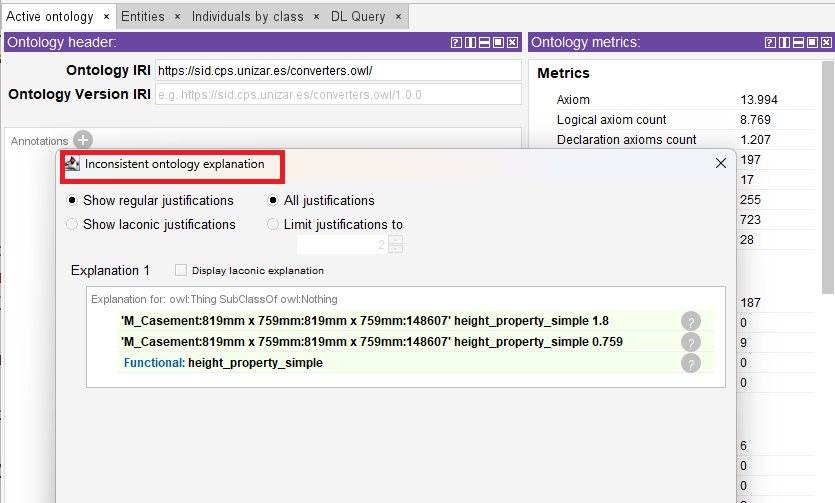
\includegraphics[width=1\linewidth,height=\textheight,keepaspectratio]{../resources/practica8/explanation.png}

}

\caption{\label{fig-explanation}Explicación de la inconsistencia
generada.}

\end{figure}%

\subsection{Descarga}\label{descarga}

\subsubsection{BIMvision}\label{bimvision}

Puedes descargar \textbf{\emph{BIMvision}} desde su
\href{https://bimvision.eu/es/descargar/}{página oficial}. Tendrás que
introducir tu correo electrónico para recibir el enlace de descarga y
aceptar los términos de servicio. Una vez hecho recibirás un correo con
el enlace para descargar el instalador. Sigue las instrucciones de
instalación para completar el proceso. Al ejecutar el programa por
primera vez, deberías ver algo como esto:

\begin{figure}

\centering{

\pandocbounded{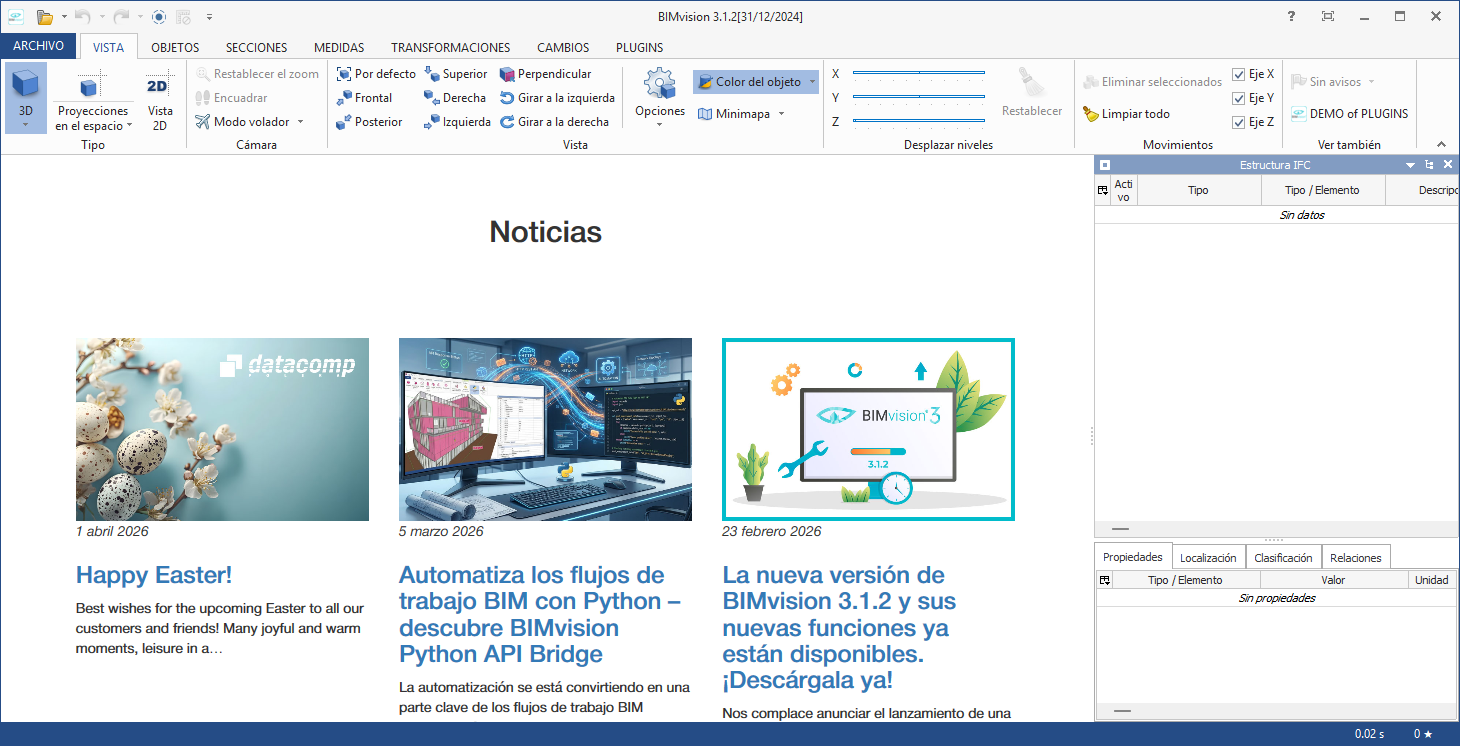
\includegraphics[keepaspectratio]{../resources/practica8/bimvision.png}}

}

\caption{\label{fig-bimvision}Pantalla de bienvenida de BIMvision.}

\end{figure}%

\subsubsection{Protégé}\label{protuxe9guxe9}

Puedes descargar \textbf{\emph{Protégé}} desde su
\href{https://protege.stanford.edu/software/\#desktop-protege}{página
oficial}. En la sección de descargas, elige la versión que corresponda a
tu sistema operativo (Windows, macOS o Linux). Descarga el archivo
comprimido y descomprímelo en una ubicación de tu elección. Ten en
cuenta que Protégé no requiere instalación adicional, por lo que puedes
situar la carpeta descomprimida en una ubicación que recuerdes
fácilmente. Para ejecutar Protégé, simplemente abre la carpeta
descomprimida y haz doble clic en el archivo \texttt{Protege.exe} (en
Windows). Al abrir Protégé, deberías ver una pantalla de bienvenida
similar a esta:

\begin{figure}

\centering{

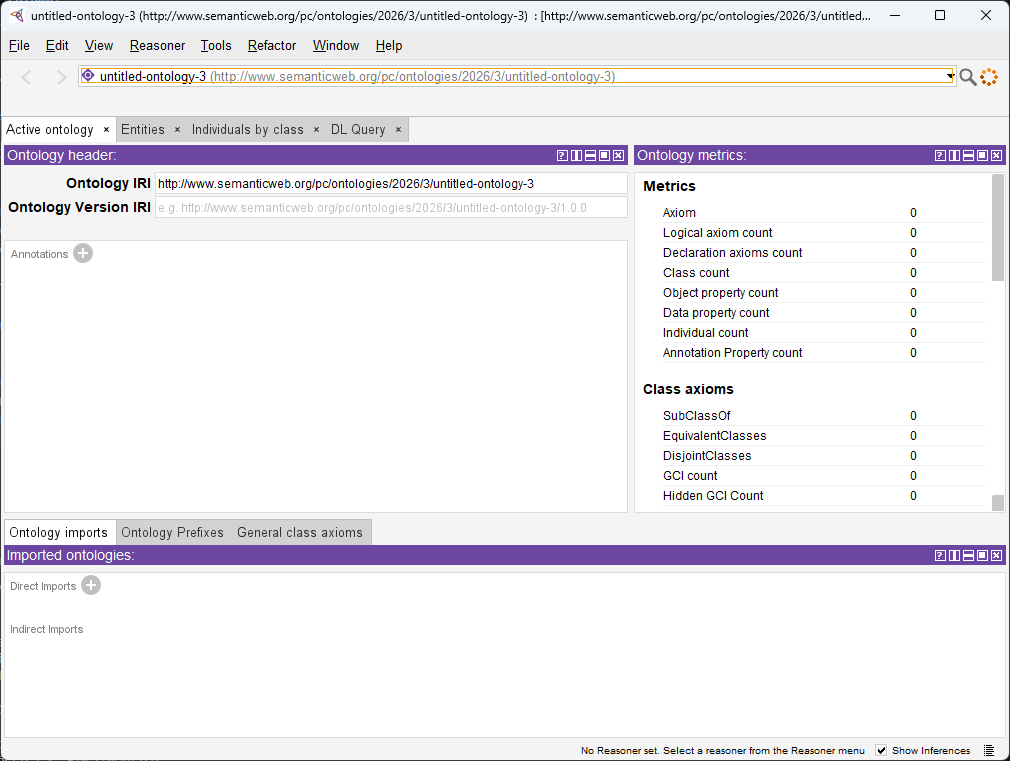
\includegraphics[width=0.8\linewidth,height=\textheight,keepaspectratio]{../resources/practica8/protege.png}

}

\caption{\label{fig-protege-welcome}Pantalla de bienvenida de Protégé.}

\end{figure}%




\end{document}
